% Chapter XY

\chapter{Supplementary Data} % Main chapter title

\label{Results} % For referencing the chapter elsewhere, use \ref{Chapter2} 

% \lhead{Chapter 2. \emph{Methods}} % This is for the header on each page - perhaps a shortened title

%----------------------------------------------------------------------------------------
\section{The phosphoserine-rich N-VP2 of MVM facilitates nuclear targeting and contributes to cytotoxicity.}


\renewcommand{\thefigure}{S\arabic{figure}}
\setcounter{figure}{0}

In order to investigate a possible involvement of the distal serine phosphorylations within N-VP2 in MVM egress, we generated a mutant, referred to as 5SG, having the corresponding serine residues substituted by glycine. In Figure~\ref{S1}, p.~\pageref{S1} several aspects of an infection with 5SG, such as cytotoxicity, nuclear targeting, and nuclear export are summarized.

\begin{figure}
\centering
  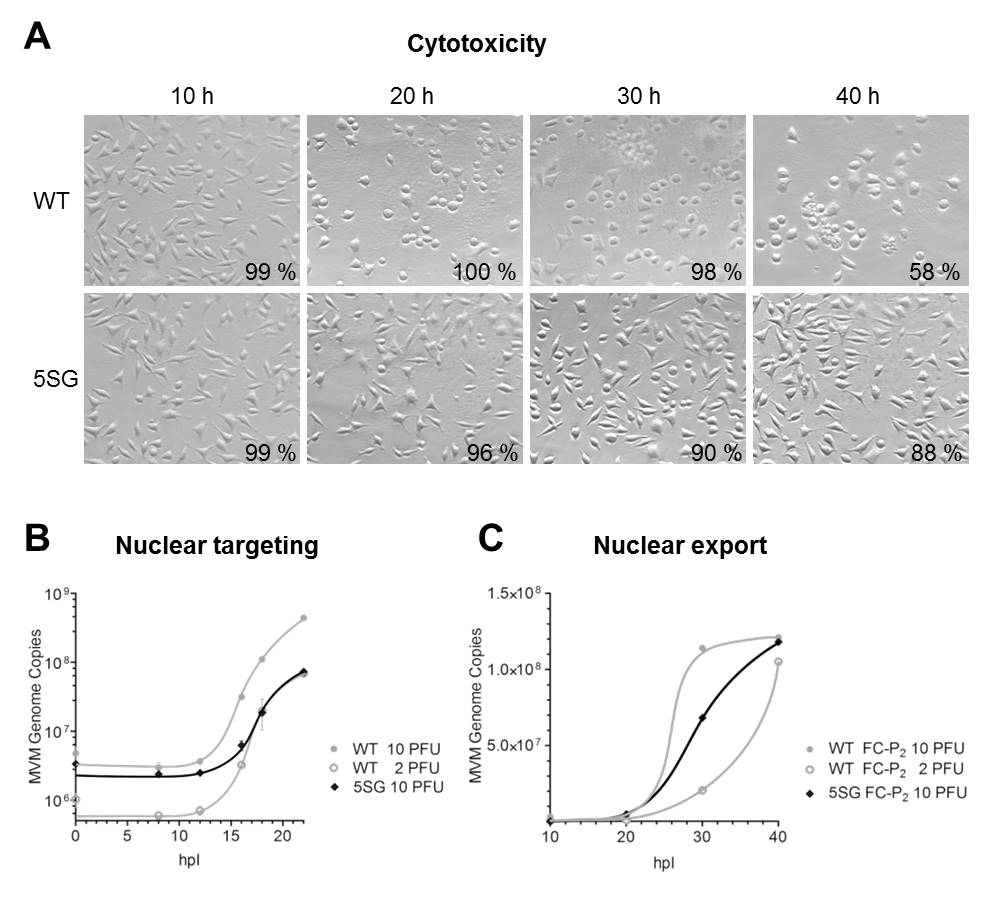
\includegraphics[scale=0.9]{S1}
  \caption[Kinetics of nuclear export depends on the input virus.]
   {\textbf{Kinetics of nuclear export depends on the input virus. (A)} A9 cells were infected with WT or 5SG MVM using 10 PFU per cell. Following binding at 4 \textcelsius~unbound virus was removed by washings. Cells were incubated at 37 \textcelsius~for the indicated times. Phase contrast pictures of the infected cells were taken using a 20$\times$ magnification objective built in a Zeiss Axiovert 35 microscope. Cell viability was accessed via trypan blue exclusion using the TC10\textsuperscript{\texttrademark} automated cell counter (BioRad). The average of three independent measurements is indicated. \textbf{(B)} A9 cells (8 $\times$ 10\textsuperscript{3}) were infected with the indicated PFU of WT or 5SG virus. Following binding at 4 \textcelsius~unbound viruses were removed. Viral DNA was extracted and quantified at the indicated times post-infection. \textbf{(C)} A9 cells (3 $\times$ 10\textsuperscript{6}) were infected using the indicated viruses and PFU. Binding was performed at 4 \textcelsius. Unbound virus was removed prior to incubation at 37 \textcelsius~for the indicated times. Cytosolic fractions were isolated and applied for AEX-qPCR. Exported FC-P\textsubscript{2} virions were quantified using qPCR. All infections were performed in the presence of $\alpha$-capsid mAb (B7) and neuraminidase in order to prevent re-infections.} 
\label{S1}
\end{figure}



In a WT infection, the cells showed reorganization of the cytoskeleton as early as 20 hpi, resulting in a rounded phenotype of affected cells. At later times, increasing amounts of cells became rounded and partially detached showing apoptotic bodies at 40 hpi, eventually resulting in cell death and cytolysis (see Figure~\ref{S1} A, 1\textsuperscript{st} row, p.~\pageref{S1}). In contrast, 5SG virions were significantly less cytotoxic. Even as late as 40 hpi most of the infected cells still exhibited the typical fibroblastic phenotype and only a few cells became rounded. No signs of apoptosis and cytolysis were observed (see Figure~\ref{S1} A, 2\textsuperscript{nd} row, p.~\pageref{S1}). 5SG was approximately 5$\times$ less efficient in replicating viral DNA in the nucleus, indicating that fewer virions reached the nucleus, thus delivering less DNA templates to initiate viral replication. Indeed, the amount of viral DNA in the nuclei of 5SG infected cells was similar to the quantities that were obtained when the cells were infected with 5$\times$ less WT virions (see Figure~\ref{S1} B, p.~\pageref{S1}). Nuclear export of 5SG progeny was not significantly affected. Virions were efficiently exported from the nucleus even though showing a slight delay in cytoplasmic accumulation (see Figure~\ref{S1} C, p.~\pageref{S1}). This delay is obviously caused by defects in early steps of infection prior to the initiation of DNA replication, such as binding, endosomal escape, viral uptake, or nuclear targeting.


As observed, productive MVM infection produces a strong cytopathic effect in the host cell, ultimately causing cellular lysis. Such dramatic changes in the cytoskeleton filaments involve gelsolin-mediated degradation of actin fibers resulting in the generation of characteristic ``actin-patches'' \cite{pmid18704167}. While the actin filaments become destabilized, the microtubule network is maintained during the course of infection \cite{pmid15582663}. The latter observation together with the previously reported capsid-dynamin co-localization~\cite{pmid18704167} would be in agreement with a microtubule dependent egress of MVM. The little delay in nuclear targeting and the fewer amount of progeny DNA in the nucleus observed for an infection with 5SG virions (see Figure~\ref{S1} B, p.~\pageref{S1}) cannot explain the delay of the cytopathic effect of more than 20 h. N-VP2 is removed by proteolytic digestion during endosomal uptake. Hence, it is not involved in important signaling for replication or progeny morphogenesis. Additionally, it has been demonstrated that there are no significant differences in the cytoplasmic accumulation of WT and 5SG progeny virions (see Figure~\ref{S1} C, p.~\pageref{S1}). Therefore, the phosphorylations on N-VP2, which represent the only difference between the WT and 5SG progeny, are likely involved in late events mediating the rearrangement of the cytoskeleton during egress. 5SG seems to be defective for severing the actin filaments resulting in prolonged maintenance of the cytoskeleton and cell integrity. 


Similar observations have been reported by G. E. Tullis et al.~\cite{pmid1448928} for a MVM mutation affecting the sequence but not the phosphorylations within N-VP2. A 7 amino acid deletion mutant lacking the trypsin-sensitive residues 17-23 within N-VP2 was slightly defective for binding and approximately 10$\times$ deficient compared to the WT in initiating a productive infection. These results suggest that the trypsin-sensitive RVER region is important for both binding and a subsequent step prior to the onset of DNA replication. Because this mutation affects both structural proteins VP1 and VP2, it is difficult to distinguish their relative contribution to the mutant phenotype. However, the binding defect is more likely a VP2 effect since virions lacking VP1 are not defective in binding to susceptible cells \cite{pmid8416366}. In addition to its defect in cell binding, the mutant showed further limitations. Similar amounts of the 7aa deletion mutant produced approximately 10$\times$ less viral DNA in the nuclei of infected cells, suggesting that fewer mutant virions, on the average, reached the nucleus where they can initiate DNA replication. Nonetheless, those that managed to reach the nucleus, replicated normally. Equally, this mutant was delayed in escaping from the cells late in asynchronous infections. However, mutant progeny virions were efficiently transported to the media early in the infection, as well as in highly synchronized infections. Therefore, this effect might be a nonspecific defect in some aspect of cytolysis rather than a defect in an active egress mechanism. A less efficient cytolysis hampers the passive release and spread of intracellular progeny virions, thus preventing their contribution in a next round of infection. 




\subsection{Isolation and characterization of empty capsids (EC)}

As previously mentioned, DNA packaging and the recently discovered capsid surface phosphorylations are a prerequisite for the externalization of N-VP2. ECs lack both a viral genome and the late phosphorylations, thus having their N-VP2 termini buried in the interior of the capsid. Therefore, EC represent an useful tool to study the role of N-VP2 during early steps in infection, such as binding and endosomal uptake. In addition to the previously characterized FC populations (FC-P\textsubscript{1} and FC-P\textsubscript{2}), infected cells also produce a considerable amount of ECs. Due to the lack of DNA, EC band at lower density compared to FC following differential centrifugation in CsCl. While FC entered the gradient to a density of 1.46 gcm\textsuperscript{-3}, EC already banded at 1.32 gcm\textsuperscript{-3}, as determined by refractometry (see Figure~\ref{S2} A, p.~\pageref{S2}). A quantitative PCR analysis of the corresponding fractions confirmed that viral DNA containing particles were depleted from ECs to almost a thousand times (see Figure~\ref{S2} B, p.~\pageref{S2}). Approximately half of the overall viral progeny population represents ECs. Therefore, it is of interest to characterize their role during the course of infection. First of all, we verified their N-VP2 conformation and the binding specificity to SA moieties. In Figure~\ref{S2} C and D, p.~\pageref{S2} it is shown that N-VP2 is not accessible to specific antibodies and proteolytic digestion by chymotrypsin (CHT), respectively. Figure~\ref{S2} E and F, p.~\pageref{S2} demonstrates that both EC and FC specifically bind to SA moieties on the surface of murine A9 cells. Binding of both capsid species can be efficiently prevented by pre-treatment of A9 cells using neuraminidase (Neur) at doses higher than 50 U/mL. These results confirm that both capsid species bind to the same receptor molecules on the surface of susceptible murine cells.           


 



\begin{figure}
\centering
  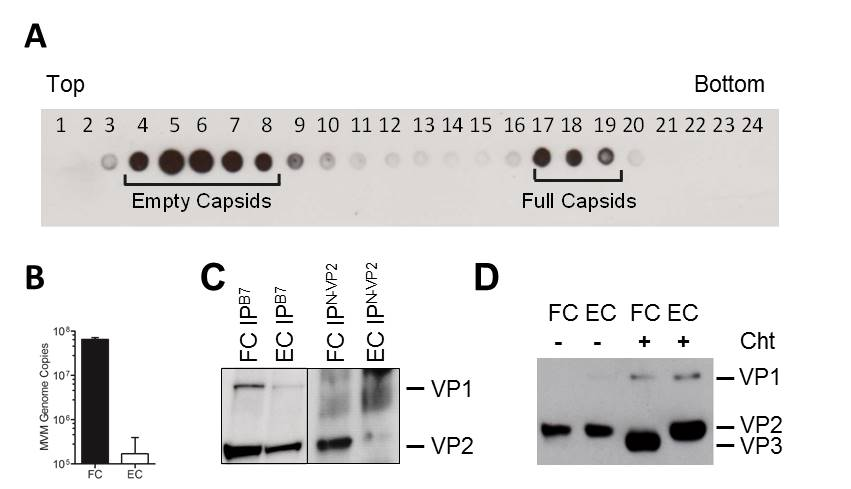
\includegraphics[scale=0.9]{S2}
  \caption[Purification and analysis of FC and EC.]
   {\textbf{Purification and analysis of FC and EC. (A)} FC and EC were separated by differential centrifugation through a CsCl gradient as described in Section~\ref{CsCl}, p.~\pageref{CsCl}. Fractions (500 $\mu$L each) are labeled from top to bottom of the gradient. 2 $\mu$L of each fraction were spotted on a nitrocellulose membrane and probed with an $\alpha$-capsid mAB (B7). A HRP-coupled secondary antibody was used and the membrane was developed by exposure to a photo film. \textbf{(B)} EC and FC fractions were pooled. qPCR analysis was performed to quantify DNA-containing particles. \textbf{(C)} N-VP2 accessibility of ECs and FCs was tested by IP using an antibody raised against the N-VP2 region. The total amount of applied viral particles was verified using an $\alpha$-capsid antibody (B7 mAb). \textbf{(D)} ECs and FCs (10\textsuperscript{8} particles each) were treated with 0.5 mg/mL chymotrypsin (CHT) or not. Proteolytic N-VP2 processing was analyzed by 10 \% SDS-PAGE. After transfer to a polyvinylidene difluoride membrane, the blot was probed with a rabbit $\alpha$-VP pAb, followed by a HRP conjugated secondary antibody. The membrane was developed by exposure to a photo film. \textbf{(E)} Following treatment with 50 U/mL neuraminidase (Neur) or not, A9 cells were infected at 4 \textcelsius~using the indicated PFU of FCs or ECs. Following washings to remove unbound viruses the cells were lysed in protein loading buffer and proteins were separated by 10 \% SDS-PAGE. Membranes were probed as outlined above. \textbf{(F)} Estimation of the effective dose of Neur in order to completely deplete MVM binding on A9 fibroblasts. Following neuraminidase treatment using the indicated doses, virus (5 PFU) was bound to 3 $\times$ 10\textsuperscript{5} cells for 1 h at 4 \textcelsius. Unbound virus was removed by washings, DNA was extracted and viral DNA was quantified by qPCR.} 
\label{S2}
\end{figure}

\footnotetext[5]{ECs do not contain DNA and thus, they are not infectious. As a consequence, no PFUs can be calculated for ECs. FCs were quantified by qPCR analysis and used as ``external standards'' for dot blot analyses. ECs were quantified by spot densitometry by comparison to serial dilutions of quantified FCs.}


\section{Comparison of ECs and FCs in early virus infection}


\subsection{Both FC and EC bind specifically to SA residues on the cell surface}


\begin{figure}
\centering
  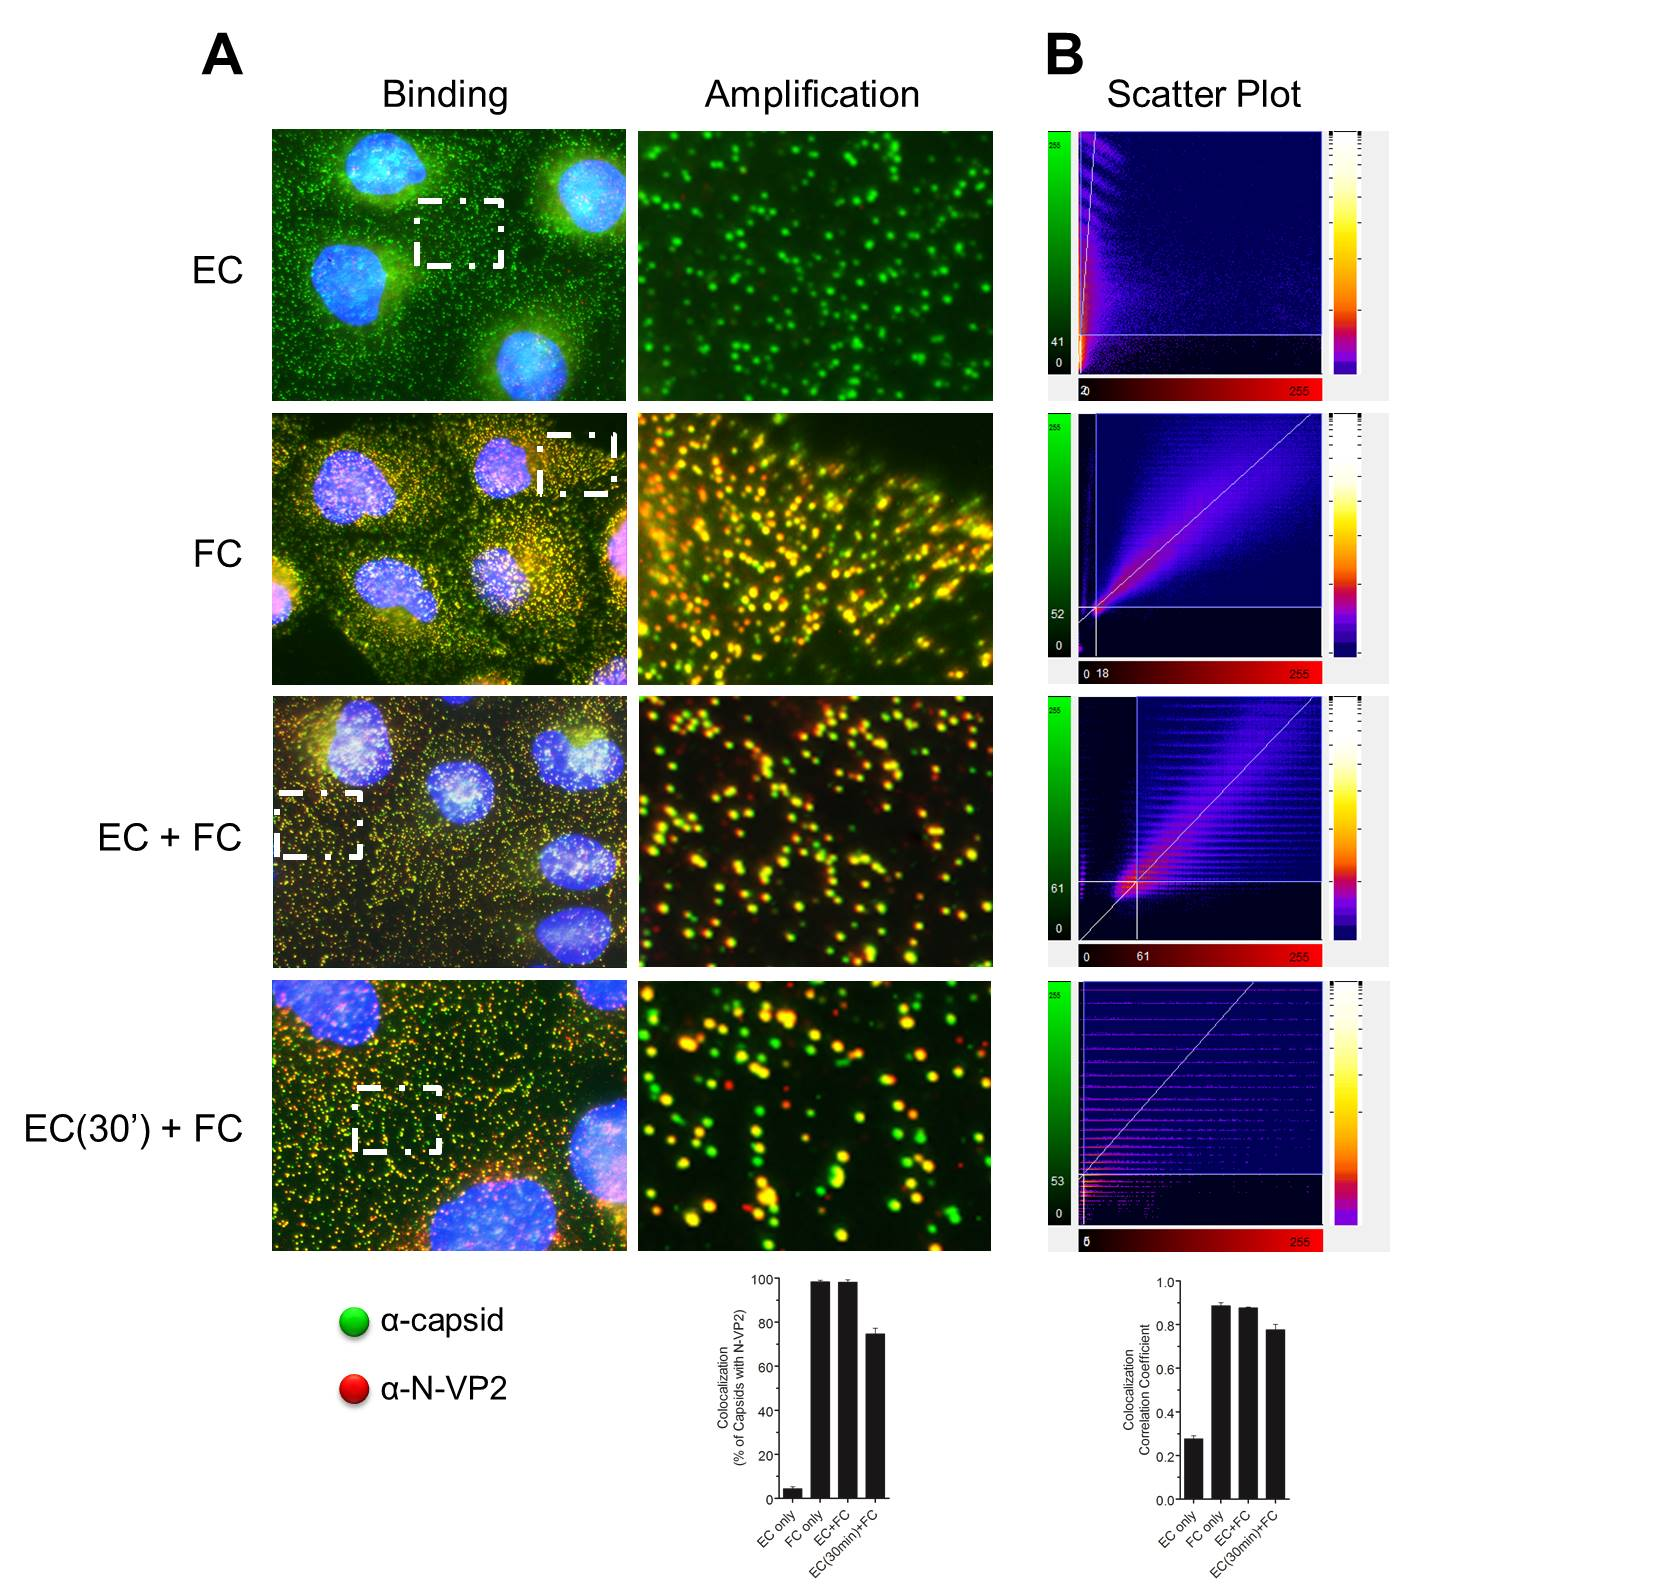
\includegraphics[width=0.95\textwidth, trim= 0mm 0mm 50mm 0mm]{S3}
  \caption[Purification and analysis of FC and EC.]
   {\textbf{FCs are preferentially bound to the SA residues on the cell surface. (A)} A9 cells (3 $\times$ 10\textsuperscript{5}) were grown on cover slips and infected independently or combined with FC and EC (5 PFU per cell) at 4 \textcelsius. In the 4\textsuperscript{th} row ECs were incubated with the cells 30 min prior to the addition of FCs. Following removal of unbound viruses the cells were fixed and stained for IF using an antibody (mAb B7) raised against assembled capsids (green) and an antibody recognizing N-VP2 (red). Percentage of capsids showing N-VP2 signal was calculated for the indicated areas of interest. (B) Scatter plots analysis showing the indicated areas of interest were used to calculate the corresponding correlation coefficient as a measurement for the degree of co-localization.} 
\label{S3}
\end{figure}

We studied their ability to bind to restrictive murine cells, their capacity to compete with FCs, and their potential to interfere with the progression of a natural infection.   


In order to characterize the binding specificity of FC and EC, both capsid types were allowed to bind discretely to susceptible, restrictive murine fibroblasts at 4~\textcelsius. At such low temperature, active cell-mediated uptake through endocytosis is prohibited. Unbound viruses were removed by several washings of the adherent cells. For restrictive mouse fibroblasts, binding saturation is reached at MOIs higher than \np{10000} DNA-containing particles per cell, as determined by the quantification of bound FCs to adherent cells at 4~\textcelsius. Both capsid species restrictively bind to SA residues since they can be completely depleted from the cell surface by treatment with neuraminidase (see Table~\ref{Enzymes}, p.~\pageref{Enzymes}), an enzyme that specifically hydrolyzes glycosidic linkages of neuraminic acids. Complete removal of attached viruses is even achieved under saturated conditions. In order to guarantee a complete removal of viral particles from the cellular surface, a minimal dose of 25 U/mL of the enzyme is required.   

\subsection{EC and FC exhibit morphological differences}
The flexible, unordered N-terminus of the major structural protein, VP2, shows distinct conformation in either capsid population. N-VP2 is accessible to proteolytic digestion or specific antibodies only in FC, whereas it remains inaccessible in EC, indicating important structural differences between these capsid populations. The differences for N-VP2 accessibility can be used to distinguish FCs and ECs in IF experiments. Staining of FCs results in co-localization of $\alpha$-Caps and $\alpha$-N-VP2 antibodies whereas ECs are detected only by $\alpha$-Caps antibodies.   

    


\subsection{FC are preferentially bound to the SA residues on the cell surface}
In silico quantification of co-localization in representative IF pictures revealed that binding of FCs was not disturbed in the presence of ECs. When FCs and ECs were bound to cells at equal stoichiometry, FCs preferentially bound to the cell surface, indicating a higher binding affinity for FCs compared to ECs. Co-localization of both antibodies was higher than 95 \% in the absence and in the presence of ECs, indicating that FCs bound preferentially to the cells. Even under non-saturated conditions, ECs were detected rarely when applied as mixed populations. Only when an equal amount of ECs was added prior to the FCs a slight increase in bound ECs was observed. Nevertheless, ECs did not represent 50 \% of the bound population but only reduced co-localization marginally to approximately 75 \%.           

\subsection{EC do not compete with FC for cell surface receptors}
Quantitative competition experiments under saturated conditions confirmed that increasing amounts of ECs did not disturb the attachment of FCs to the cell surface. These results substantiate the preferential binding of FCs to susceptible cells previously observed in IF experiments. Even an unnatural 16-fold excess of ECs did not significantly disturb receptor binding of FCs. 


Due to the differences in N-VP2 conformation among FCs and ECs, there is evidence that the N-VP2 termini may be involved in the stabilization of the binding   


\renewcommand\thefigure{\thechapter.\arabic{figure}} 

